
%(BEGIN_QUESTION)
% Copyright 2012, Tony R. Kuphaldt, released under the Creative Commons Attribution License (v 1.0)
% This means you may do almost anything with this work of mine, so long as you give me proper credit

Determine the amount of water consumed by a factory from day 6 to day 11, given the trend of flow measurements shown here:

$$\includegraphics[width=15.5cm]{i01889x01.eps}$$

Choose the closest answer:

\begin{itemize}
\item{} 6 units
\vskip 10pt 
\item{} 5 units
\vskip 10pt 
\item{} 15 units
\vskip 10pt 
\item{} 10 units
\vskip 10pt 
\item{} 11 units
\vskip 10pt 
\item{} 17 units
\vskip 10pt 
\item{} 14 units
\end{itemize}

\underbar{file i01889}
%(END_QUESTION)





%(BEGIN_ANSWER)

14 units

%(END_ANSWER)




%(BEGIN_NOTES)

{\bf This question is intended for exams only and not worksheets!}.

%(END_NOTES)


